%Preambolo per documento generico
%Per cambiare tipo di documento modificare
%il documentclass.

\documentclass[11pt]{article}
\usepackage[utf8]{inputenc}

%Mettere italian se si vuole scrivere in italiano
\usepackage[english]{babel}


%Aumento dell'interlinea
\usepackage{setspace}
\onehalfspacing

%Pacchetti per simboli matematici
\usepackage{mathtools}
\usepackage{amsfonts}
\usepackage{amsthm}
\newtheorem{theorem}{Theorem}
\usepackage{amsmath}
\usepackage{bm}


%Pacchetti per figure e tabelle
\usepackage{booktabs, caption, graphicx, subfig, float}
\captionsetup{tableposition=top,figureposition=bottom,font=small}

%Per inserire commenti in blocco
%Usage: \begin{comment} ... \end{comment}
\usepackage{comment}

%Definisce colori dei link nel testo e altri parametri
\usepackage{hyperref}
\hypersetup{
pdftitle={VSDProjectReport},%
pdfauthor={Carrarini,Kieffer,Tantucci,Wrona},%
pdfsubject={},%
pdfkeywords={},%
colorlinks=true,%
linkcolor=black,%
linktocpage=true,%
pageanchor=true,
citecolor=black
}

%Definisce in maniera simmetrica i margini di pagina
\usepackage{geometry}
\geometry{a4paper, top=3cm,bottom=3cm,left=3cm,right=3cm,%
			heightrounded}

%Per scrivere in maniera rapida norme e valori assoluti
%Usage: y = \abs{x} ; y = \norma{x}

\DeclarePairedDelimiter{\abs}{\lvert}{\rvert}
\DeclarePairedDelimiter{\norma}{\lVert}{\rVert}
%Testo a caso
%Usage: \lipsum[a-b] | Esempio \lipsum[1-10]
\usepackage{lipsum}

%Cambia lo stile della pagina
%In alto a dx mette numero di pagina
%In alto a sinistra titolo e autore
\usepackage{fancyhdr}
\pagestyle{fancy}
\fancyhf{}
\rhead{\textit{\thepage}}
\lhead{\textit{On KERS implementation}}

%Per inserire codice nativo MATLAB e simili
%Usage: guardare sotto
\usepackage{fancyvrb}

\usepackage[dvipsnames]{xcolor}
\definecolor{sapred}{RGB}{130,36,51} %colore sapienza per i titoli


\begin{document}

\title{\textcolor{sapred}{On KERS implementation}\\\small{Vehicle System Dynamics Project}}
\author{Luca Carrarini\\Federico Kieffer\\Andrea Tantucci\\Andrea Wrona}
%Optional: data. Se non si inserisce il campo data
%LaTeX mette la data del PC automaticamente
%\date{}
\maketitle

\thispagestyle{empty}

\tableofcontents
\newpage

%Inizio dei capitoli
\section{Introduction}

The dependence of the transportation sector on non-renewable sources of energy as fossil fuels and the need for a rapid response to the global warming challenge has in the last two decades encouraged a strong effort for the development of fuel efficient vehicle propulsion systems. In this context, a particular attention has been devoted to the concept of regenerative breaking. A regenerative brake is a mechanism that reduces the vehicle speed by converting some of its kinetic energy into some other kind of useful forms of energy, such as mechanical, electrical or hydraulic energy \cite{a}. The core devices of regenerative brakes are therefore reversible energy conversion components like electric motors/generators and hydraulic pumps/motors. For example, an electric regenerative brake makes use of an electric motor that acts as a generator. This device, which is usually made integral with the vehicle wheel trough a gear train, is indeed able to generate electrical energy thanks to the inputted kinetic energy that is associated to the vehicle at the end of any acceleration phase. 
A type of regenerative braking is called KERS. KERS, which stands for Kinetic Energy Recovery System, is an automotive system for recovering a moving vehicle's kinetic energy under braking. The recovered energy is stored in a reservoir, as for example a flywheel, a battery or a super capacitor, for later use under acceleration \cite{b}. 
Embedding such a system in a vehicle allows several potential advantages. First of all, KERS systems may be included in the class of \textit{energy harvesting} devices \cite{c}, which are likely to have a consistent impact in the scenario of \textit{green technologies} and \textit{environment-friendly} solutions. In fact, the partial regeneration of the energy that is usually dissipated by the service brake in conventional systems may allow impactful fuel economy strategies, thus reducing the fossil fuel demand and the consequent green-house gases (CO2) emissions. Another important advantage that such a system introduces is the reduced service brake wear. In fact, since during regenerative brakes an electric/hydraulic motor is used to slow down the vehicle in place of the conventional disk brake, this component will benefit from a longer lifetime. 

\section{Implementation alternatives}

In this section, we give a description and a comparison of the principle KERS systems that have been proposed in the literature and on the market.

\subsection{Mechanical KERS}

\subsubsection{Architecture and working principle}

The Flywheel Hybrid System (FHS) is a type of KERS which consists of a rotating mass, or flywheel, as the energy storage device, a continous variable transmission system (CVT) to control and transfer the energy to and from the driveline and a clutch which connects this system to the primary shaft of the transmission (\figurename\,\ref{fig: FHS}). 

\begin{figure}[H]
\centering
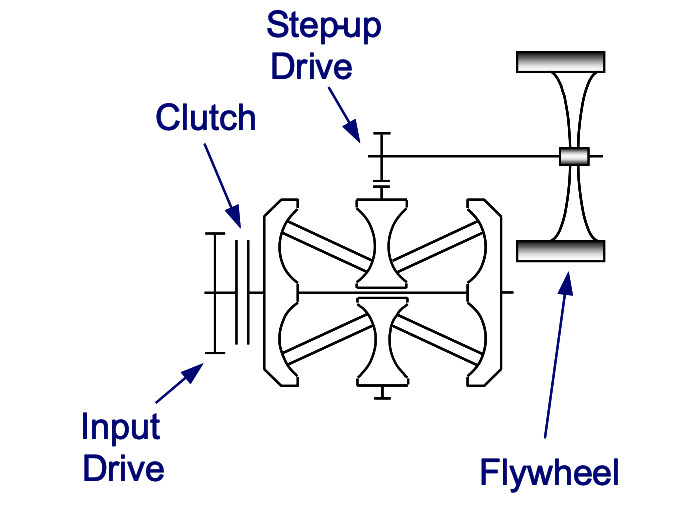
\includegraphics[width=.6\textwidth]{Images/Mechanical_KERS.png}
\caption{Schematic of Flywheel Hybrid System}
\label{fig: FHS}
\end{figure}

When the brakes are applied or the vehicle decelerates, the clutch connecting the flywheel system to the driveline/transmission is engaged, causing energy to be transferred to the flywheel via the CVT. \\
The use of the CVT guarantees a smooth transfer of energy thanks to the fact that it has an infinite number of gear ratios between the maximum and minimum value of the speed. The Toroidal CVT must continuously adjust the ratio between the speed of the vehicle and the rotation of the flywheel. Any change in the CVT ratio can be viewed as the transfer of kinetic energy between the flywheel inertia and vehicle.\\
The flywheel stores this energy as rotational energy and can rotate up to a maximum speed of $60000$ rpm. When the vehicle stops, or the flywheel reaches its maximum speed, the clutch disengages the flywheel unit from the transmission allowing the flywheel to rotate independently. Whenever this stored energy is required, the clutch is engaged and the flywheel transmits this energy back to the wheels, via the CVT. To optimise efficiency, the flywheel runs in a high vacuum and is enclosed within a housing that provides containment in the event of failure.
The major function of the vacuum chamber is to minimize the air resistance as the flywheel rotates. Without the vacuum chamber, the friction caused by air resistance is enough to cause significant energy losses and heat the carbon fibre rim to its glass transition temperature. In \figurename\,\ref{fig: Flywheel} we can see the design of a flywheel.\\
Another important part of the system are the bearings on which the flywheel is mounted. Magnetic bearings have replaced mechanical bearings as they greatly reduce losses due to friction. Further magnetic bearings are able to operate in vacuum which leads to even better efficiency. The magnetic bearings support the flywheel by the principle of magnetic levitation. It is important that the bearings are able to operate inside a vacuum because the flywheel in a flywheel-based KERS must rotate at high speeds for maximum efficiency. The best performing bearing is the high-temperature super-conducting (HTS) magnetic bearing.

\begin{figure}[H]
\centering
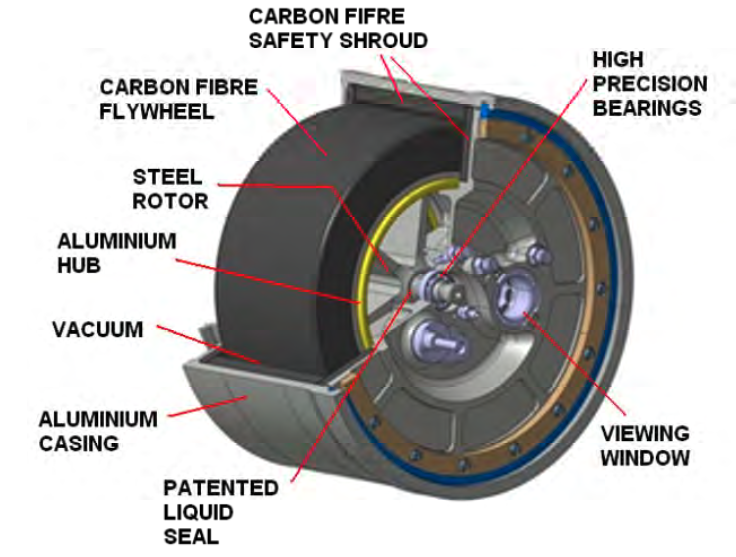
\includegraphics[width=.6\textwidth]{Images/Flywheel_Components.png}
\caption{Section of the flywheel}
\label{fig: Flywheel}
\end{figure}

We have also the presence of a step--up gearing system consisting of epicyclic gears is connected between the CVT and the flywheel unit. This system is used to reduce the speed of the flywheel to a manageable one outside the vacuum chamber, in order to have a smooth transfer of energy to the CVT.\\
The clutch instead is used to couple the flywheel hybrid system to the transmission. It engages the system while the flywheel is accelerating from rest and disengaging while the flywheel is rotating and the vehicle is at rest. Torque is transferred through clutch between the flywheel and vehicle. Hence, the power transmitted in the flywheel system can be controlled by a clutch that could continuously manipulate the torque.

\subsubsection{Advantages, disadvantages and fields of application}

The advantages include high efficiency, low fuel consumption, and low cost compared to electric hybrids. Although the system has a few drawbacks, most of it can be outweighed by the benefits. One main advantage of this KERS system is its weight. Due to the lightweight design of the flywheel and accompanying components, the additional weight is insignificant when analysing fuel efficiency. Moreover, the system is contained in a compact package, making it easy to incorporate into the rear of a vehicle. Another advantage is the ability of the flywheel to store energy efficiently. This is because there is no transformation of energy from one form to another which greatly reduces energy losses in the system. Tests have proven that flywheel--based KERS can recover and store over $70\%$ of the vehicle’s energy. Probably the only losses that occur in the system might be due to friction and air resistance to the flywheels rotation. However, the magnetic bearings and vacuum chamber mentioned previously have been developed to minimize these effects. Cars with a flywheel based energy recovery system, though significantly more expensive than cars without this system, have more power and better fuel efficiency. It has been proved that the system could reduce fuel consumption by as much as $20$\% and give a four-cylinder engine acceleration like a six-cylinder unit.\\
The system has low maintenance costs and it reduces break wear.\\
As with any technology, the flywheel KERS system has its shortcomings as well. The flywheels found in a kinetic energy recovery system can store up to $400$ kJ of energy, which means that failure while rotating at $60000$ rpm could cause immense amounts of damage. The flywheel--based KERS is not designed to be a stand-alone source of power for a vehicle, like batteries are in electric cars. It is designed for temporary energy storage that is to be used frequently and in smaller amounts. Its purpose is to reduce fuel consumption by providing additional power during the acceleration of a vehicle. Periods of acceleration, especially from a stop, are when the efficiency of the vehicle is at its lowest.


\subsection{Electric KERS}

Electric KERS is a type of KERS which makes use of batteries or/and supercapacitors as storage system. This regenerative brake system can be used both in the case of internal combustion engine, electric vehicle and hybrid vehicle.

\subsubsection{Architecture and working principle}

There are different implementations in literature of electric KERS (e-KERS) and each architecture is more suitable for particular application. In Fig.\ref{ekersdrivetrainuc} e-KERS with supercapacitor as principal and unique storage system is described. The scheme is composed by: the supercapacitor (SC) which is the energy storage part of the system, it is electrically interfaced to the motor-generator unit (MGU) through power converter (PC). MGU is connected to drive shaft. 

\begin{figure}[H]
	\centering
	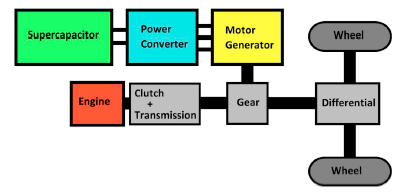
\includegraphics[width=.6\textwidth]{Images/Electric_KERS_uconly.PNG}
	\caption{Drivetrain layout with e-KERS}
	\label{ekersdrivetrainuc}
\end{figure}
 
\begin{figure}[H]
	\centering
	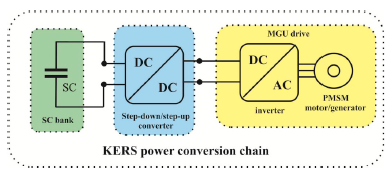
\includegraphics[width=.6\textwidth]{Images/Electric_KERS_scheme_uconly.PNG}
	\caption{E-kers scheme}
	\label{ekersschemeuc}
\end{figure}

There exists also the dual of this implementation which is the one in which there are only batteries used as storage system. These two implementations have several limitations. SC as single energy storage element can be used only when large spaces and weight were allowed (i.e. electric city rail, hybrid city bus). Batteries have high energy density(Li-ion batteries, that are the most installed batteries on electric vehicle, have specific energy density around 75–200Wh/kg) but low power density. For automotive applications, specifically in hard braking and traction maneuvers, batteries present several weaknesses related to the chemical reactions taking place while charging/discharging. Li-Ion batteries cannot respond to high-dynamic power profiles resulting from an acceleration or a regenerative
braking since charge transfer occurs through reduction and oxidation reactions. These profiles, if happened, will overstress the batteries which negatively affect the longevity of their lifespan. It is convenient to implement in the energy storage system, a storage element characterized by its ability to provide the necessary power required by the traction and braking systems. This secondary storage element will substitute the battery during extreme power demand. Among all the existing storage elements, the supercapacitors are potential candidates to meet those requirements. This element has high power density and high cycle life. On the other hand, it presents a low energy density, a high acquisition cost and a high self-discharge. The hybrid energy storage system (HESS) will combine the high energy density storage element (Li-Ion battery), known as primary storage element, and the high power density storage element (supercapacitor). HESS implementation is described in Fig.\ref{ekersschemehybrid}

\begin{figure}[H]
	\centering
	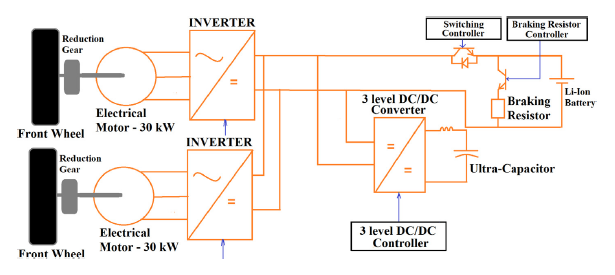
\includegraphics[width=.6\textwidth]{Images/Electric_KERS_scheme_hybrid.PNG}
	\caption{Hybrid e-kers scheme}
	\label{ekersschemehybrid}
\end{figure}

It is possible to see in Fig.\ref{ekersschemepowerflow} the power flow from wheel to storage system during brake phase.

\begin{figure}[H]
	\centering
	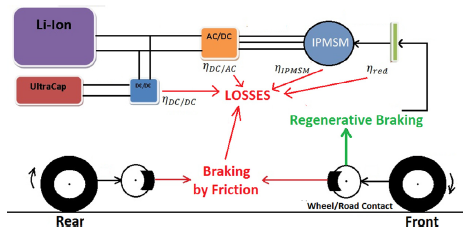
\includegraphics[width=.6\textwidth]{Images/Electric_KERS_powerflow.PNG}
	\caption{Hybrid e-kers scheme}
	\label{ekersschemepowerflow}
\end{figure}


\subsubsection{Advantages, disadvantages and fields of application}

It is possible to evaluate and to compare electrical energy storage system by using some performance metrics like the cycle efficiency, the cost per unit capacity(\$/kWh or \$/kW), specific energy (Wh/kg), specific power (W/kg) ,energy density (Wh/l), power density (W/l), cycle life. The battery has shorter cycle life due to unavoidable chemical deterioration. No single type of electrical energy storage element can simultaneously fulfill all the desired characteristics. There will be a need to combine higher energy density insured by the battery, as primary source, with a higher power density energy storage elements, like ultracapacitors or flywheel. This means that the best e-KERS implementation is the hibrid one which makes use of primary and secondary source. The use of supercapacitor as unique storage solution in electric vehicles remains limited since their energy density cannot compete with batteries. It is possible to use only supercapacitors as storage system if a low driving range can be accepted and if there is enough space available to install supercapacitors and when there are no weight constraints as in the case of electric city rail or hybrid city bus, where energy saving of about $40\%$ were obtained. Both HEV  and FCHEV  usually implement electric KERS, exploiting the main storage system used for the traction in conjunction with supercapacitors, which allow a reduction of batteries intervention during vehicle regenerative braking or startup, thus enhancing batteries life cycle and maintaining their capacity performance. Regenerative braking has been intensively studied and implemented on hybrid electric vehicles (HEV) and fuel cell hybrid electric vehicles (FCHEV) because the presence of powerful electric machines (generator and motor) interfaced to high capacity energy storage as batteries easily allows to convert and store vehicle kinetic energy into electric energy. Stored energy can be employed for vehicle propulsion or for electronic components supply.  Stationary flywheels have important dimensions and excessive weight. Onboard flywheels need space in the bogie requiring more space than ultracapacitors. After the diffusion of UCs, the use of flywheels in electrified railways has been reduced because of the superior properties of UCs in terms of maintenance, weight and size [21]. Other authors conclude that flywheel ensures a steady voltage and power level, which is independent of load, temperature and state of charge. In fact the combination battery/flywheel can achieve better performance, regarding voltage fluctuation, than other types of combinations (battery/UC or UC/flywheel), as reported by [46]. Unlike electrified vehicles, internal combustion engine vehicles are not equipped with generator, electric motor and batteries of adequate power and capacity to allow the conversion of the vehicle kinetic energy into electric energy. For this reason, the kinetic energy recovery systems successfully tested for ICEV application are mainly based on mechanical and hydraulic energy storage devices. Unfortunately, the energy recovered through the flywheel cannot be stored for a long time, due to mechanical and fluid dynamics friction on the flywheel.
 

\subsection{Hydraulic KERS: Series Hydraulic Hybrid systems}

Series Hydraulic Hybrid Systems(SHH) represent a type of KERS that makes use of hydraulic accumulators as energy storage units. Unlike the older \textit{parallel} implementations, the \textit{series} architecture is characterized by the fact that prime-mover and vehicle speeds are entirely decoupled through a continuously variable hybrid hydraulic transmission. In other words, the conventional mechanical driveline is completely removed.

\subsubsection{Architecture and working principle}

The system (fig. 1) is made of four principal components \cite{d} the working fluid (usually oil), the ICE, hydro-pneumatic accumulators and pumps/motors, which are often variable displacement axial piston machines.

\begin{figure}[H]
\centering
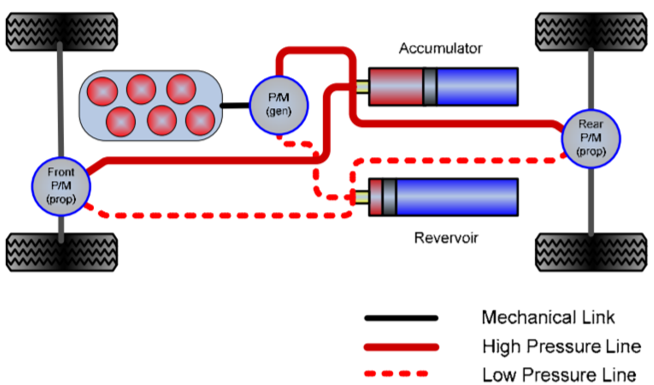
\includegraphics[width=.6\textwidth]{Images/Hydraulic KERS.png}
\caption{SHH scheme for a 4x4 vehicle}
\label{StepF1}
\end{figure}

The IC engine is mechanically coupled to the hydraulic pump/motor designated as P/M(gen). The P/M(gen) is used as a motor only when starting the engine. In all the other working conditions, the fluid pumped by P/M(gen) flows towards the P/M(prop-s) and the high pressure accumulator. Traction pumps/motors (P/Mprop-s) are connected to the wheels through a differential to provide propulsion. The pump/motor is a reversible energy conversion component. In particular, operating the P/M(prop) in the motor mode propels the vehicle, while regenerative braking requires switching to the pump mode. During the breaking phase, the hydro-pneumatic accumulator allows energy storage: as the P/M(prop), working as a pump, transfers the hydraulic fluid from the reservoir into the accumulator, the pressure of the gas sealed inside it increases, thus storing energy \cite{e}. In the accumulator (fig. 2), a bladder is used to separate the working fluid from the pressurized inert gas (e.g. nitrogen), which can be thus treated as a closed system. In a later acceleration event, the energy stored in the high pressure fluid contained in the accumulator is used, together with an amount delivered by the P/M(gen), to provide torque to the wheels. The pressure difference between the accumulator and the reservoir determines the maximum torque available from the hydraulic motor. In this phase, the working fluid is at least partially returned to the reservoir. 

\begin{figure}[H]
\centering
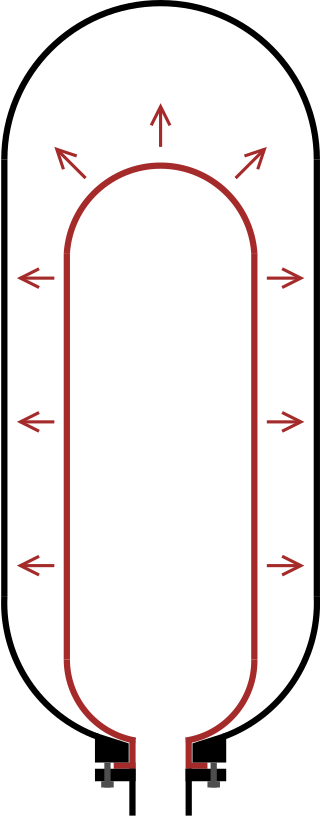
\includegraphics[width=.1\textwidth]{Images/Hydraulic Accumulator.png}
\caption{Bladder-type hydraulic accumulator}
\label{StepF1}
\end{figure}

The Reservoir is structurally similar to the accumulator but the gas that it contains is kept at low pressures and serves primarily to assist the transfer of fluid to-and-from the accumulator, with a minimal impact on the overall energy conversion. 

\subsubsection{Advantages, disadvantages and fields of application}

In contrast to its electric counterpart, fluid power technology is characterized by a higher power density and lower energy density \cite{f}. Energy density, which is also known as specific energy, represents the amount of energy that can be stored in a given mass of the system. On the other hand, energy density does not give information on how quickly this energy can be used: this knowledge is contained in the system's power density, which describes the rate at which its energy can be outputted. Moreover, since they release their energy more quickly, higher power density systems can also recharge more quickly. This feature makes hydraulic hybridization particularly interesting for applications with high and fast power transients.  In particular, utilization of hydraulic propulsion and energy storage components can offer significant advantages for those heavy vehicles that are required frequent start-stop operations, such as city buses, delivery vehicles and refuse trucks. It’s worth noticing that, in those fields of application, the stored energy is not necessarily limited to aid subsequent acceleration events, but can potentially represent a power source for the activation of ancillary equipment, as for example the compacting and packing mechanisms of refuse trucks. In addition, hydraulic KERS are also likely to have a longer operating life than battery-powered systems.  Another remarkable advantage of those systems is their high energy conversion efficiency: the state-of-the art bladder type accumulators with elastomeric foam can reach a round-trip efficiency of about 95\%. Once again, the combination of high efficiency and high charging-discharging rates enables particularly effective regeneration and re-use of hydraulic energy in heavy vehicles.
The main disadvantage of hydro-pneumatic KERS is represented by their high weight, which is mainly due to the presence of the working fluid and accumulators. This causes the specific energy of those systems to be relatively low. As a result, hydraulic hybrid systems encounter important limitations where consistent levels of power are required for extended periods at near constant speeds, such as in long-distance cruising.
Additional costs, which may represent 10–15\% of the total for the vehicle, is undoubtedly a further important drawback.

\subsection{Hydro-electric KERS}




%Codice per inserire le figure
\begin{comment}
\begin{figure}[H]
\centering
\includegraphics[width=.6\textwidth]{Charts/StepF1}
\caption{Step response of the closed--loop relative to $F_1$}
\label{StepF1}
\end{figure}
\end{comment}


%Codice per inserire il codice
\vspace{4cm}
This is a fancy in--line code
\singlespacing
\begin{Verbatim}[tabsize = 4, frame = lines, numbers = left]
code_here...
	code_here...
code_here...
\end{Verbatim}
\onehalfspacing


\begin{thebibliography}{3}
	
	%%%
	
	%GENERAL STRUCTURE FOR THE BIBLIOGRAPHY
	
	%Cognome, Nome appuntato, (Anno), Nome del paper o del libro, Editrice o rivista, città (Stato), pagine.
	
	%Esempio
	%Kapoor R., Parveen C. M., (2013), \textit{Comparative %Study on Various KERS}, Proceedings of the World Congress %on Engineering 2013 Vol III, London.
	
	%%%
	\bibitem{a}
	J. Chibulka , “Kinetic Energy Recovery system by means of Flywheel Energy 		    storage device”. 
	Advanced Engineering, vol. 3, issue 1, pp. 27-38, 2009.
	
	\bibitem{b}
	R. Chicurel, “A Compromise Solution for Energy Recovery in Vehicle Braking”.      	Energy, vol.24, pp. 1029-1034, 2009.
	
	\bibitem{c}
	A. Harb. “Energy harvesting: State-of-the-art”. 
	Renewable energy, vol. 36, pp. 2641-2654, 2011.
	
	\bibitem{d}
	K. Baer et Al. “Robustness and performance evaluations for simulation-based 		control and component parameter optimization for a series hydraulic hybrid 			vehicle”,  Engineering Optimization 2020, VOL. 52, NO. 3, 446–464.	
	
	\bibitem{e}
	Y. J. Kim et Al., “Simulation Study of a Series Hydraulic Hybrid Propulsion 		System for a Light Truck”. SAE International, 2007.
	
	\bibitem{f}
	M. Shan “Modelling and Control Strategy for Series Hydraulic Hybrid 				Vehicles”.  PhD thesis, 2009.
	
	\bibitem{g}
	D. Nishanth, T. Mathews "Flywheel based Kinetic Energy Recovery System(KERS) integrated in vehicles". International Journal of Engineering Science and Technology (IJEST), Vol. 5 No.09 Sep 2013.
	
	\bibitem{h}
	Pipitone, Emiliano, and Gianpaolo Vitale. "A regenerative braking system for internal combustion engine vehicles using supercapacitors as energy storage elements-Part 1: System analysis and modelling." Journal of Power Sources 448 (2020): 227368.
	
	\bibitem{i}
	Itani, Khaled, et al. "Comparative analysis of two hybrid energy storage systems used in a two front wheel driven electric vehicle during extreme start-up and regenerative braking operations." Energy Conversion and Management 144 (2017): 69-87.
	
	\bibitem{l}
	Kapoor R., Parveen C. M., (2013), \textit{Comparative Study on Various KERS}, Proceedings of the World Congress on Engineering 2013 Vol III, London.
	
	\bibitem{m}
	Hui S., Lifu Y., Junqing J., (2010), \textit{Hydraulic/electric synergy system (HESS) design for heavy hybrid vehicles}, Energy 35, pp. 5328--5335.
	
	
\end{thebibliography}

\end{document}
